% !TeX spellcheck = en_US
% !TeX program = pdflatex

\documentclass{beamer}
\usepackage[utf8]{inputenc} % russian, do not change
\usepackage[T2A, T1]{fontenc} % russian, do not change
\usepackage[english, russian]{babel} % russian, do not change

% fonts
%\usepackage{fontspec} % different fonts
%\setmainfont{Times New Roman}
\usepackage{setspace,amsmath}
\usepackage{amssymb} %common math symbols
\usepackage{dsfont}

% utilities
\usepackage{systeme} % systems of equations
\usepackage{mathtools} % xRightarrow, xrightleftharpoons, etc
\usepackage{array} % utils for tables
\usepackage{makecell} % multirow for tables
\usepackage{subfiles}
\usepackage{hyperref}
\hypersetup{pdfstartview=FitH,  linkcolor=blue, urlcolor=blue, colorlinks=true}
\usepackage{framed} % advanced frames, boxes
\usepackage{graphicx}
\usepackage{caption}
\usepackage{subcaption} % captions for subfigures
\usepackage{color}
\usepackage{chngcntr} % change counters
%\counterwithout*{section}{chapter} % continue sections enumeration with chngcntr


% styling
\usetheme{default}
\usepackage{float} % force pictures position
\floatstyle{plaintop} % force caption on top
\usepackage{enumitem} % itemize and enumerate with [noitemsep]
\setlength{\parindent}{0pt} % no indents!

% misc
\graphicspath{{./img/}}
\newcommand{\myPictWidth}{.95\textwidth}
\newcommand{\phm}{\phantom{-}}
\newcommand{\defeq}{\overset{def}=}

\title{A Survey on Graph Kernels}
\subtitle{Kriege, Nils M. et al, Applied Network Science, 2020}
\author{Валерий Зуев}
\begin{document}
\begin{frame}[plain]
    \maketitle
\end{frame}
\begin{frame}{Кратко о графах}

\begin{align*}
    & G \defeq (V, E), E \in V \times V \text{ -- (неориентированный) граф } \\
    & \text{\emph{помеченный} граф } \defeq \exists l: V(G) \to \Sigma, \Sigma \text{ -- алфавит (например, } \mathds R ^d \text{) } \\
    & \text{окрестность } N(\nu) \defeq \{ u \in V(G) | (v, u) \in E(G) \}
\end{align*}

Граф можно задать матрицей смежности, матрицей инциденции, лапласианом.

\end{frame}

\begin{frame}{Кратко о ядрах}

Пусть область определения входных данных $ X $ -- непустое множество (например, $ \mathds{R}^d $ или множество конечных неориентированных графов).
Пусть $ K: X \times X \to \mathds R $.

$ K $ ядро $ \overset{def}\Leftrightarrow $
\[\exists \left(H_K, \phi: X \to H_K \right): K(x,y) = <\phi(x), \phi(y)> \forall x,y \in X \]
Можно доказать, что $ K $ ядро $ \Leftrightarrow $ $ K $ -- положительно полуопределённая функция.

\end{frame}

\begin{frame}{Свёрточные ядра}

$R$-свёрточное ядро:

\begin{itemize}[label={$\triangleright$}]
    \item Рассмотрим $ x \in X, x $ состоит из частей $\vec x = \{ x_1, \dots, x_d \}, x_i \in X_i $ (то есть задано бинарное отношение $ R : X_1 \times \dots \times X_d \times X \to \{true, false \} $).

    \item $ R^{-1}(x) \defeq \{ \vec x: R(\vec x, x) \} $

    \item $ K(x,y) \defeq \sum_{\vec x \in R^{-1}(x), \vec y \in R^{-1}(y)} \prod_{i=1}^{d} K_i(x_i, y_i) $

    \item Теорема: если $ K_1, \dots, K_d $ -- ядра в пространствах $ X_1 \times X_1, \dots, X_d \times X_d $, то при определённых разумных ограничениях $ K $ -- ядро в $ X \times X $
\end{itemize}

Haussler D (1999) Convolution kernels on discrete structures. Tech. Rep. UCS-CRL-99-10
\end{frame}

\begin{frame}{Пример свёрточного графового ядра}
	\begin{enumerate}[label=$\triangleright$]
		  \item Vertex Label Kernel
		\[ K_{VL}(G,H) \defeq \sum_{u \in V(G)} \sum_{v \in V(H)} K(l(u, l(v))) \]
		  \item Edge Label Kernel -- то же самое, но для рёбер
	\end{enumerate}
\end{frame}

\begin{frame}{Графовые ядра}
	\begin{enumerate}[label=$\triangleright$]
		\item Подходы на основе агрегации соседей
		\[ ] l^{i}: V(G) \cup V(H) \to \Sigma, i = 0, 1, \dots \]
		\[ l^i(\nu) = relabel\left( l^{i-1}(\nu), \text{sort}(\{ l^{i-1}(u) | u \in N(\nu) \}) \right), \nu \in V_G \cup V_H \]
		% TODO написать в подсказку
		\pause
		\item Подходы на основе поиска совпадений
		
		Optimal assignment kernel: $ ] G, H $ -- графы с представлениями вершин $ \{g_i\}, \{h_j\} $.
		\[ K_A(G,H) = \max_{\pi \in permutations(\{1,\dots,n\})} \sum_{i=1}^{n} K(g_i, h_{\pi(i)}) \]
		\pause
		\item Паттерны подграфов
		\item Обходы и пути
	\end{enumerate}
\end{frame}

\begin{frame}{Пример подхода на основе агрегации соседей: WL}
\begin{center}
 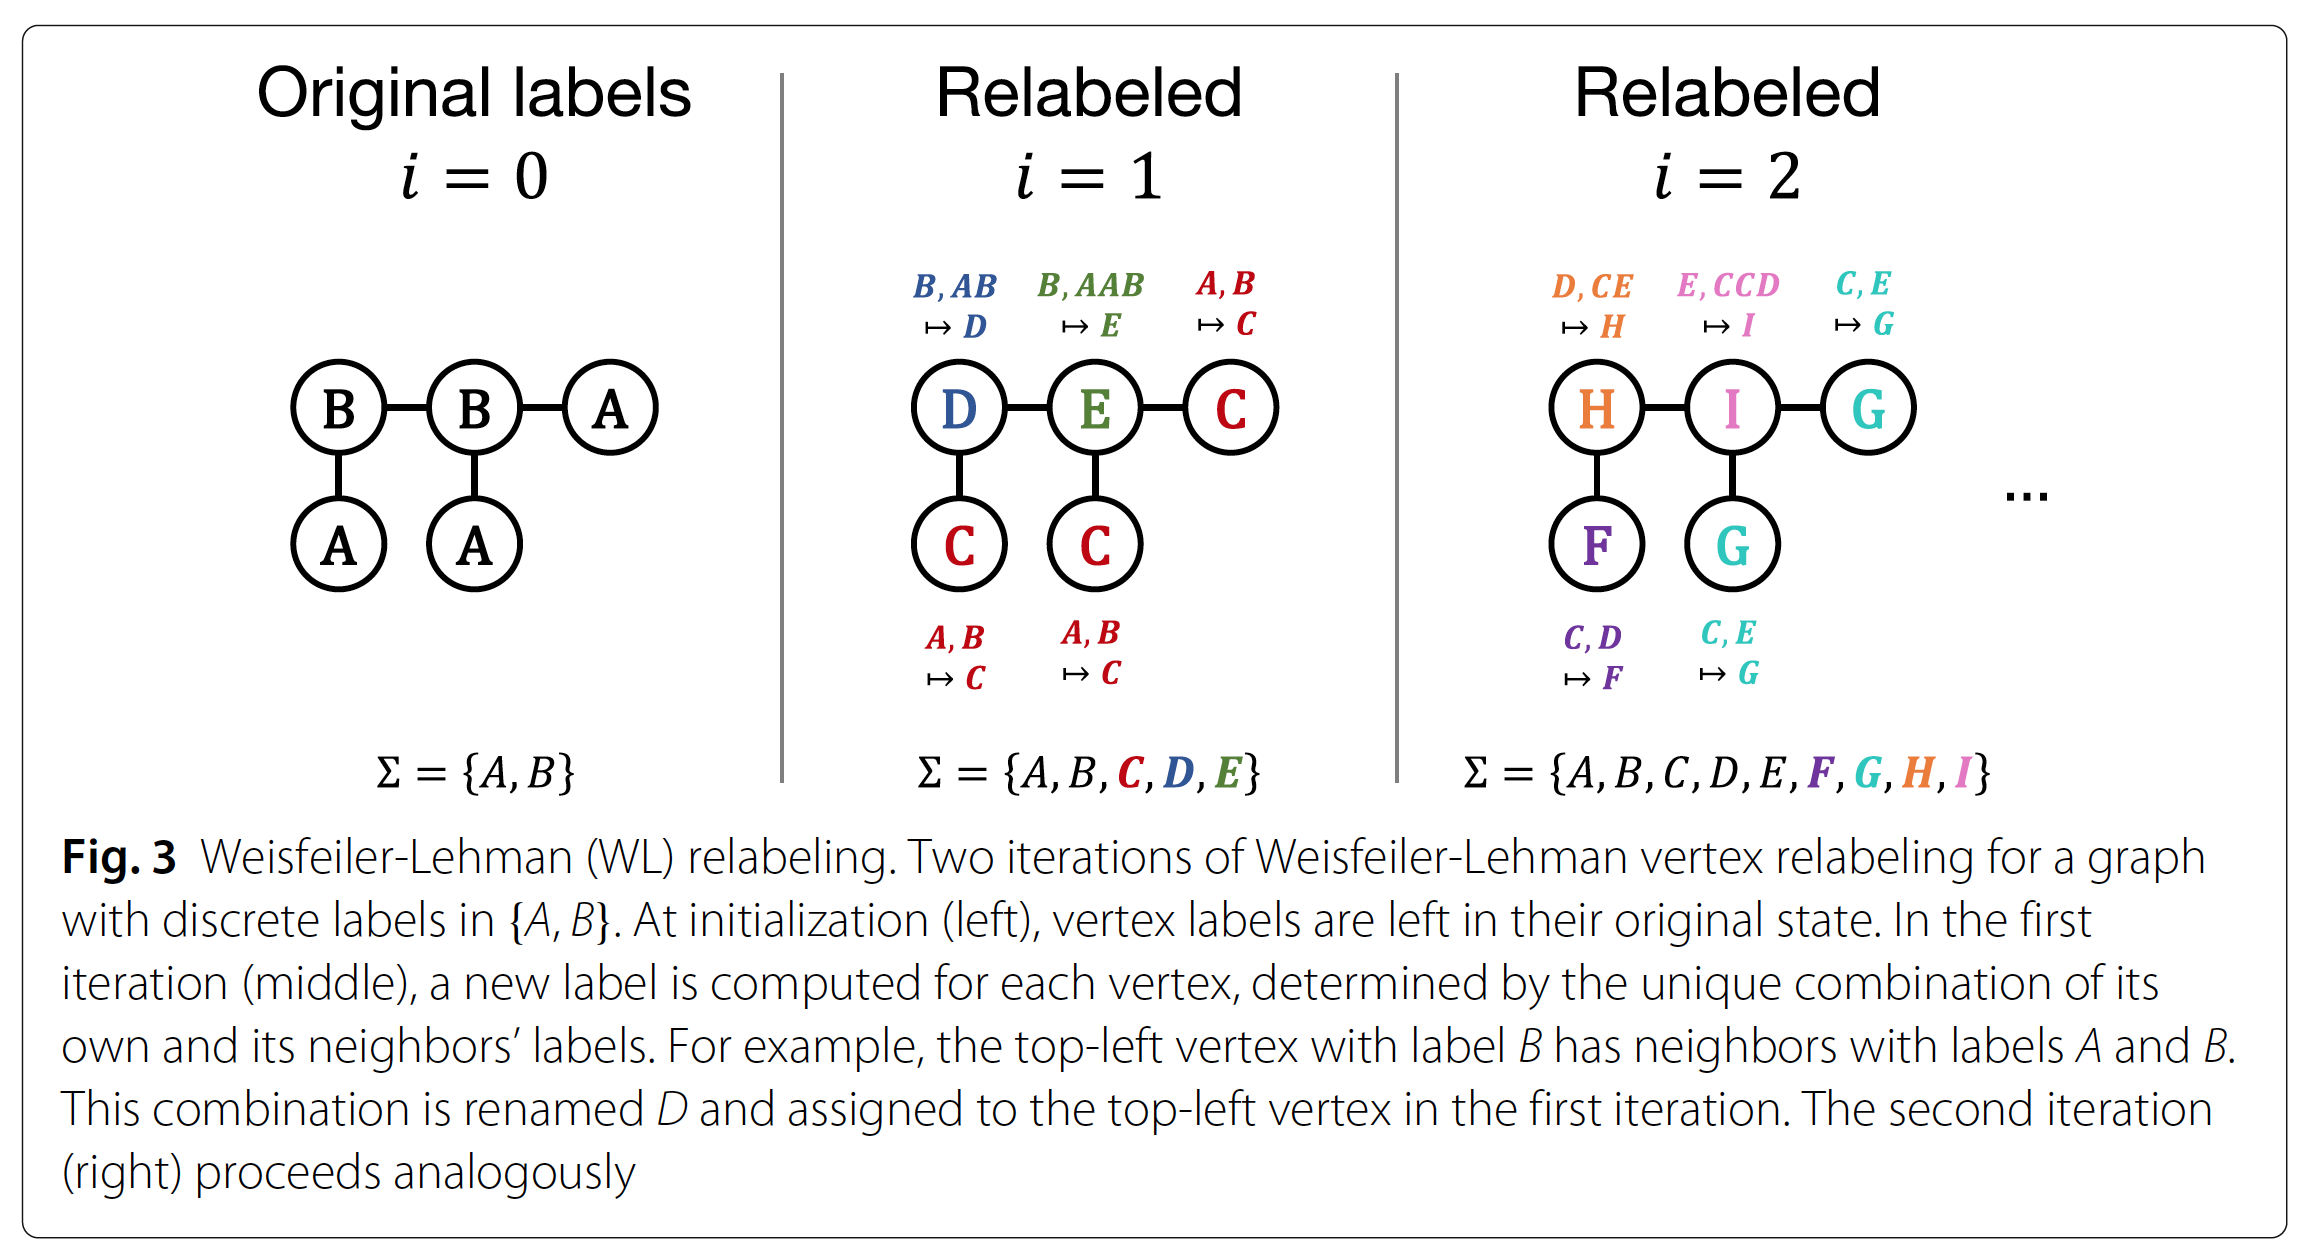
\includegraphics[width=\textwidth]{wl}
\end{center}

Shervashidze N et al (2011) Weisfeiler-Lehman graph kernels.
J Mach Learn Res 12:2539–2561

\end{frame}

\begin{frame}{Пример подхода на основе поиска совпадений: OA}
	\begin{center}
		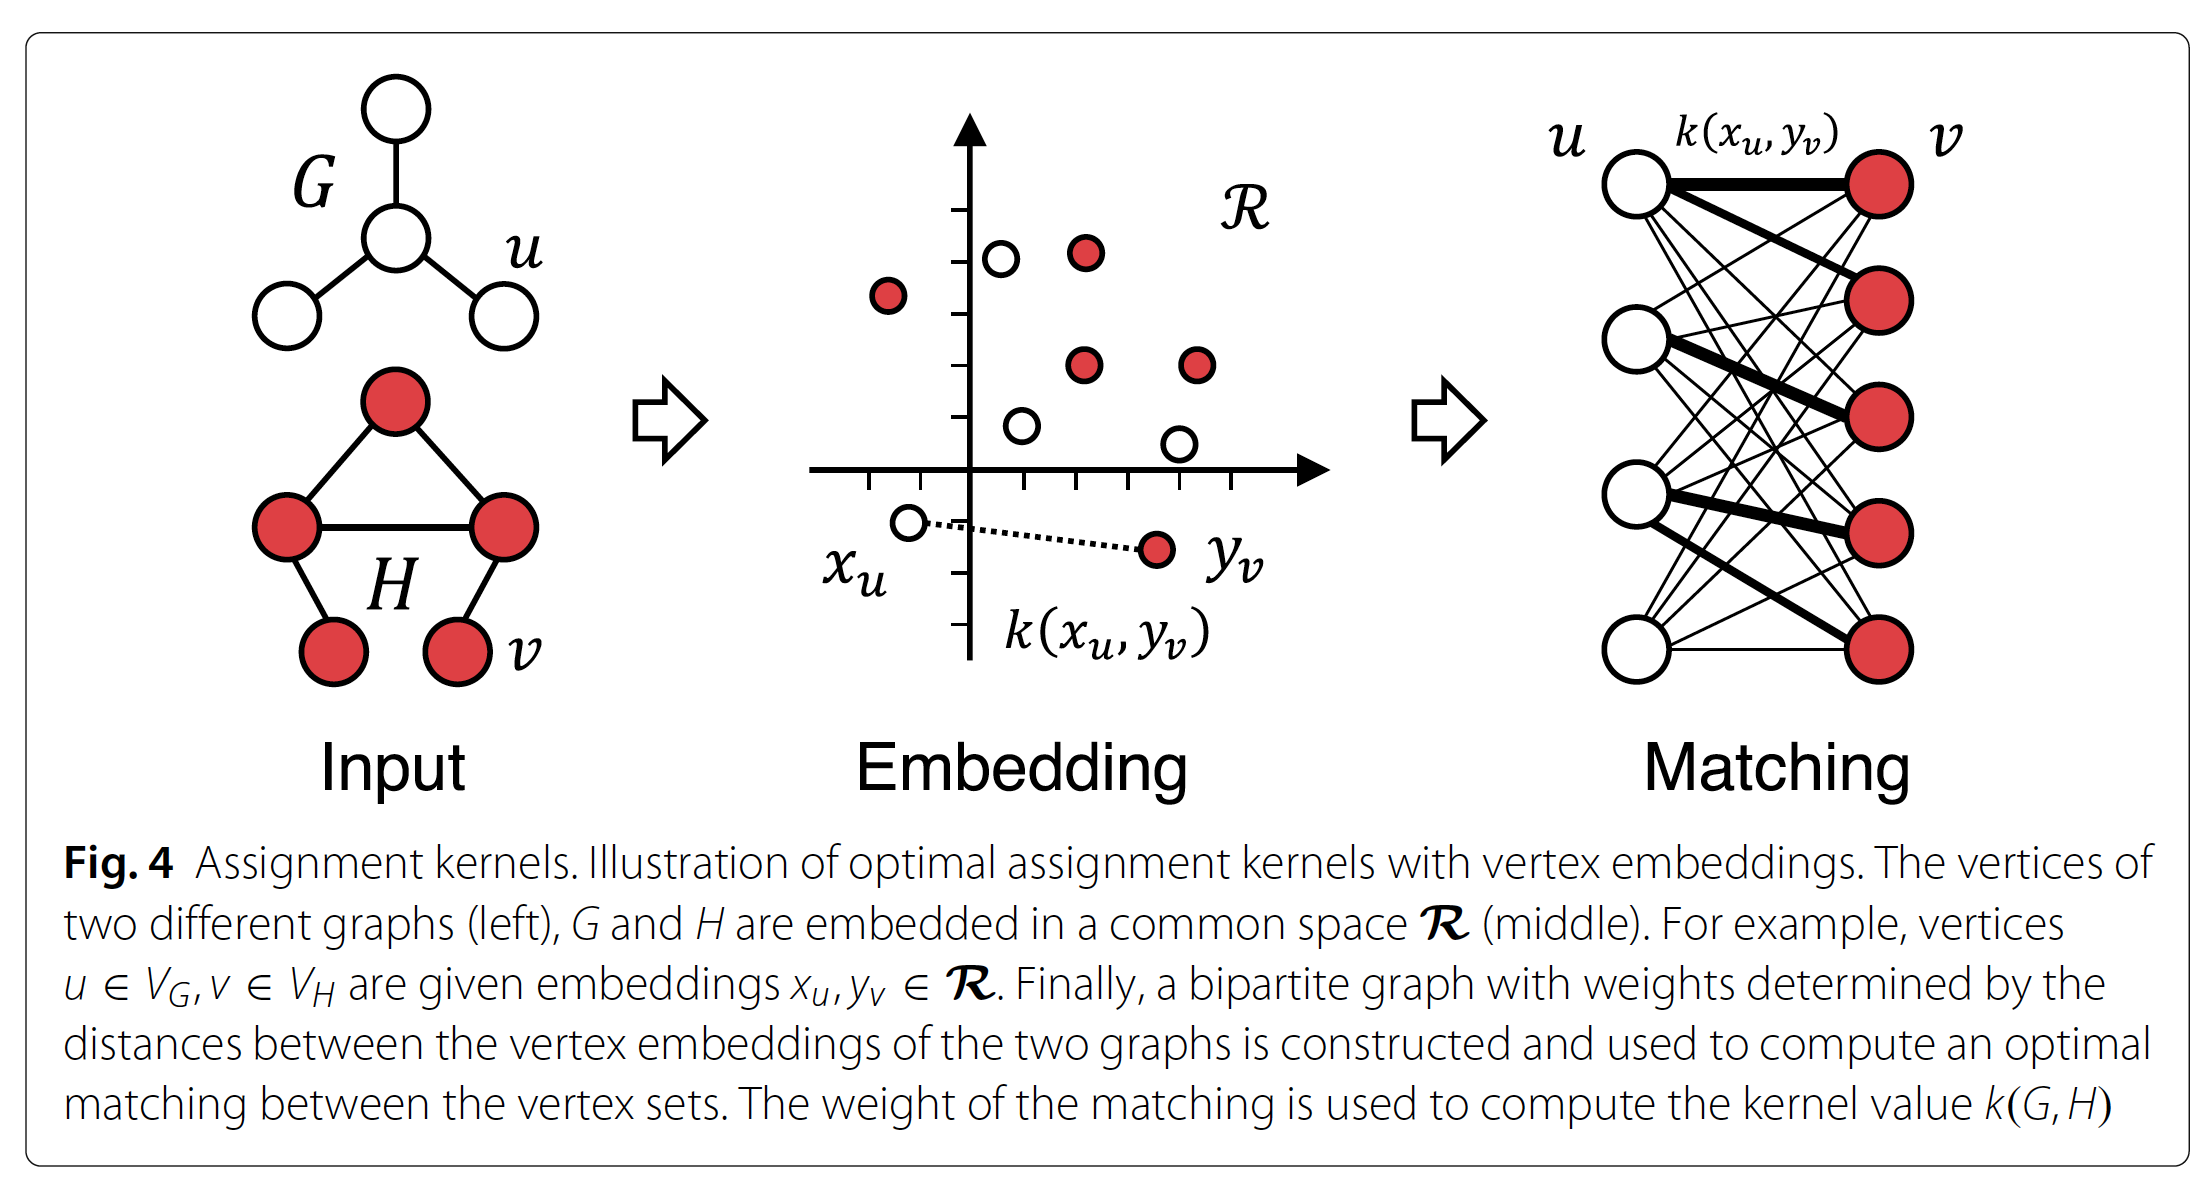
\includegraphics[width=\textwidth]{oa}
	\end{center}
	
\end{frame}

\begin{frame}{Пример подхода на основе сравнения подграфов: графлеты}
	\begin{center}
		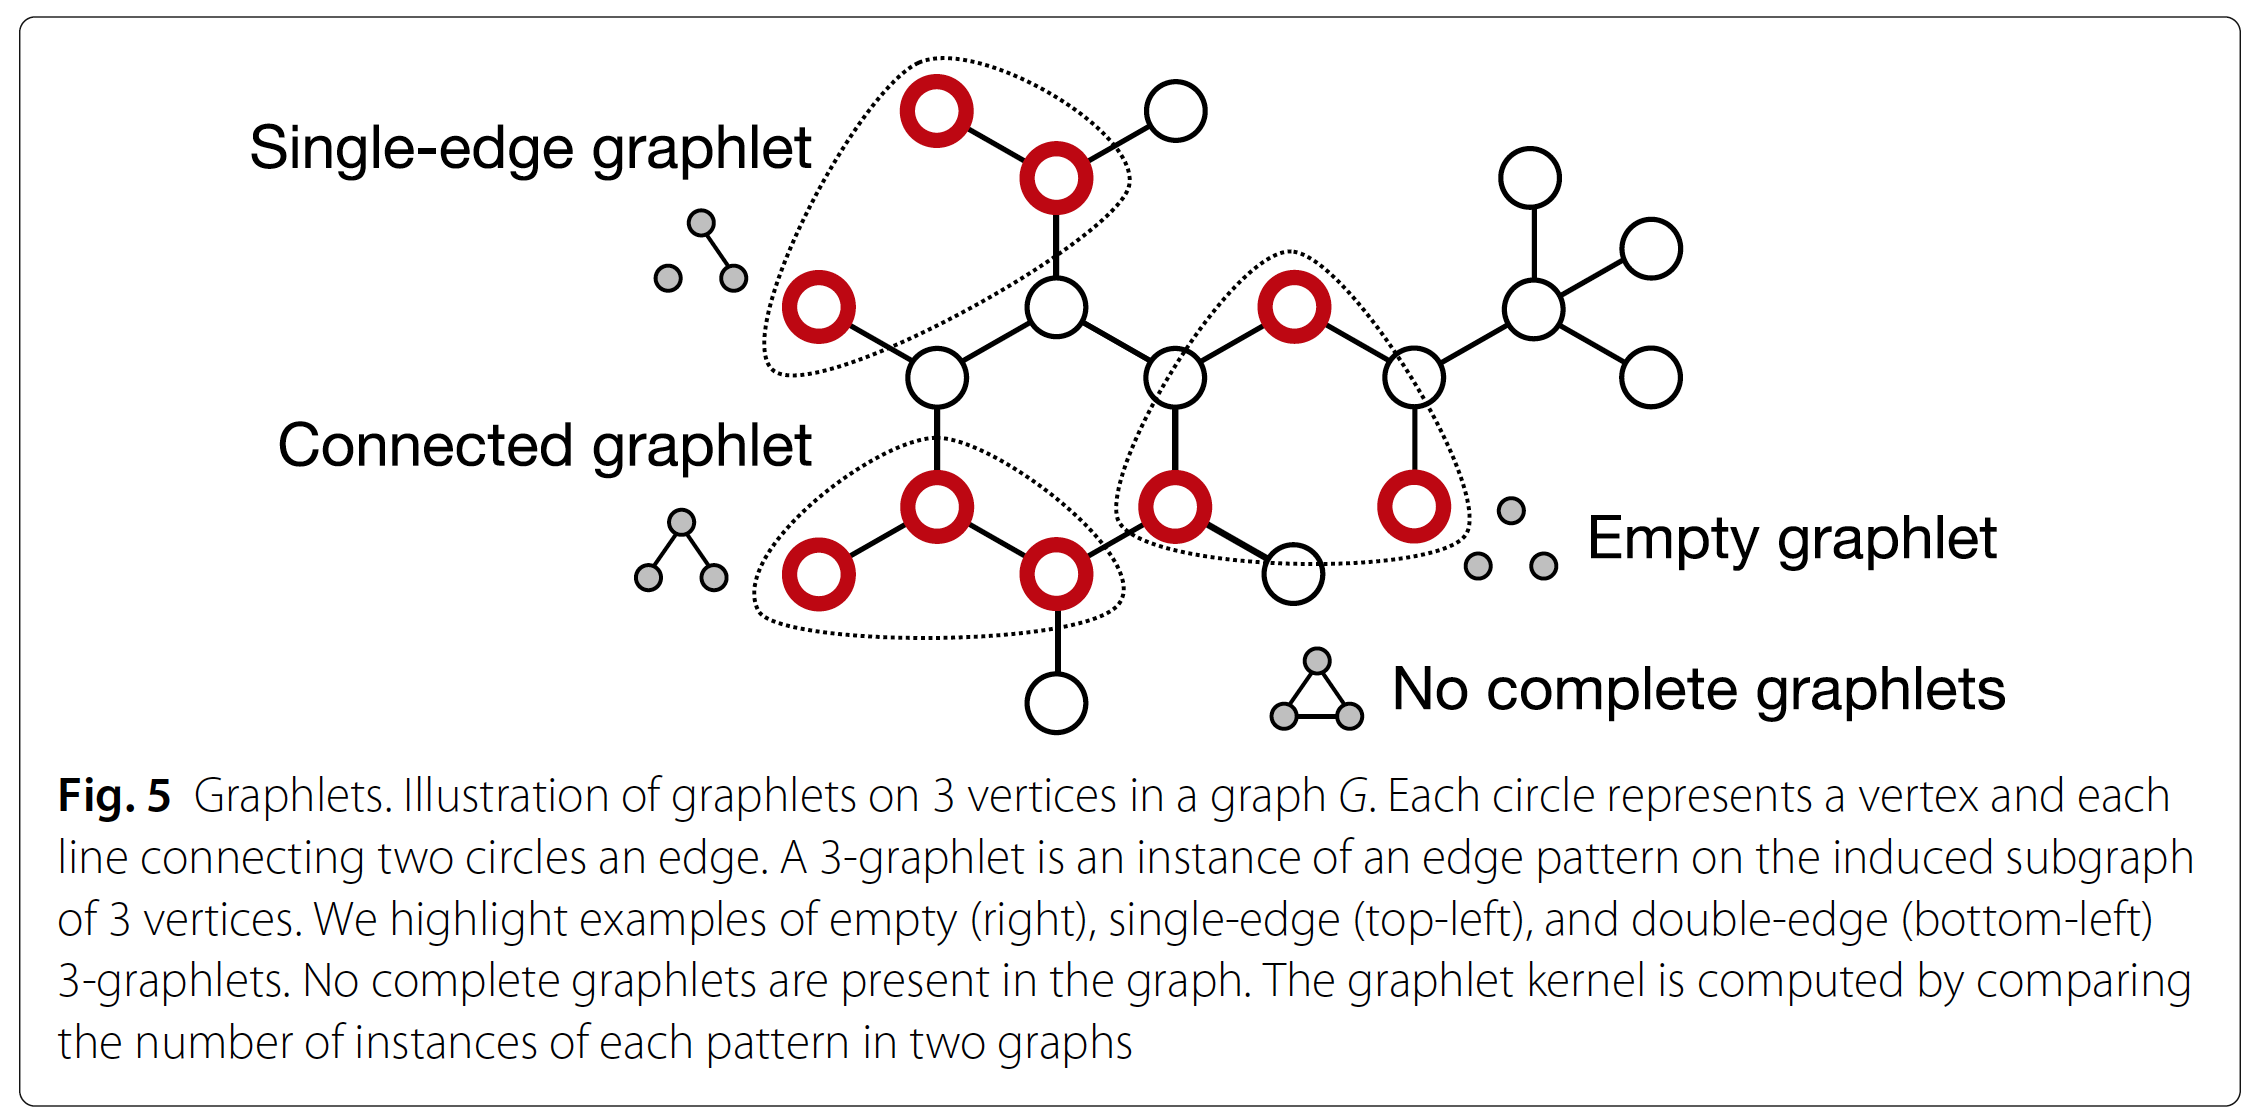
\includegraphics[width=\textwidth]{graphlet}
	\end{center}
	
\end{frame}

\begin{frame}{Пример подхода на основе путей: прямое произведение}
	\begin{center}
		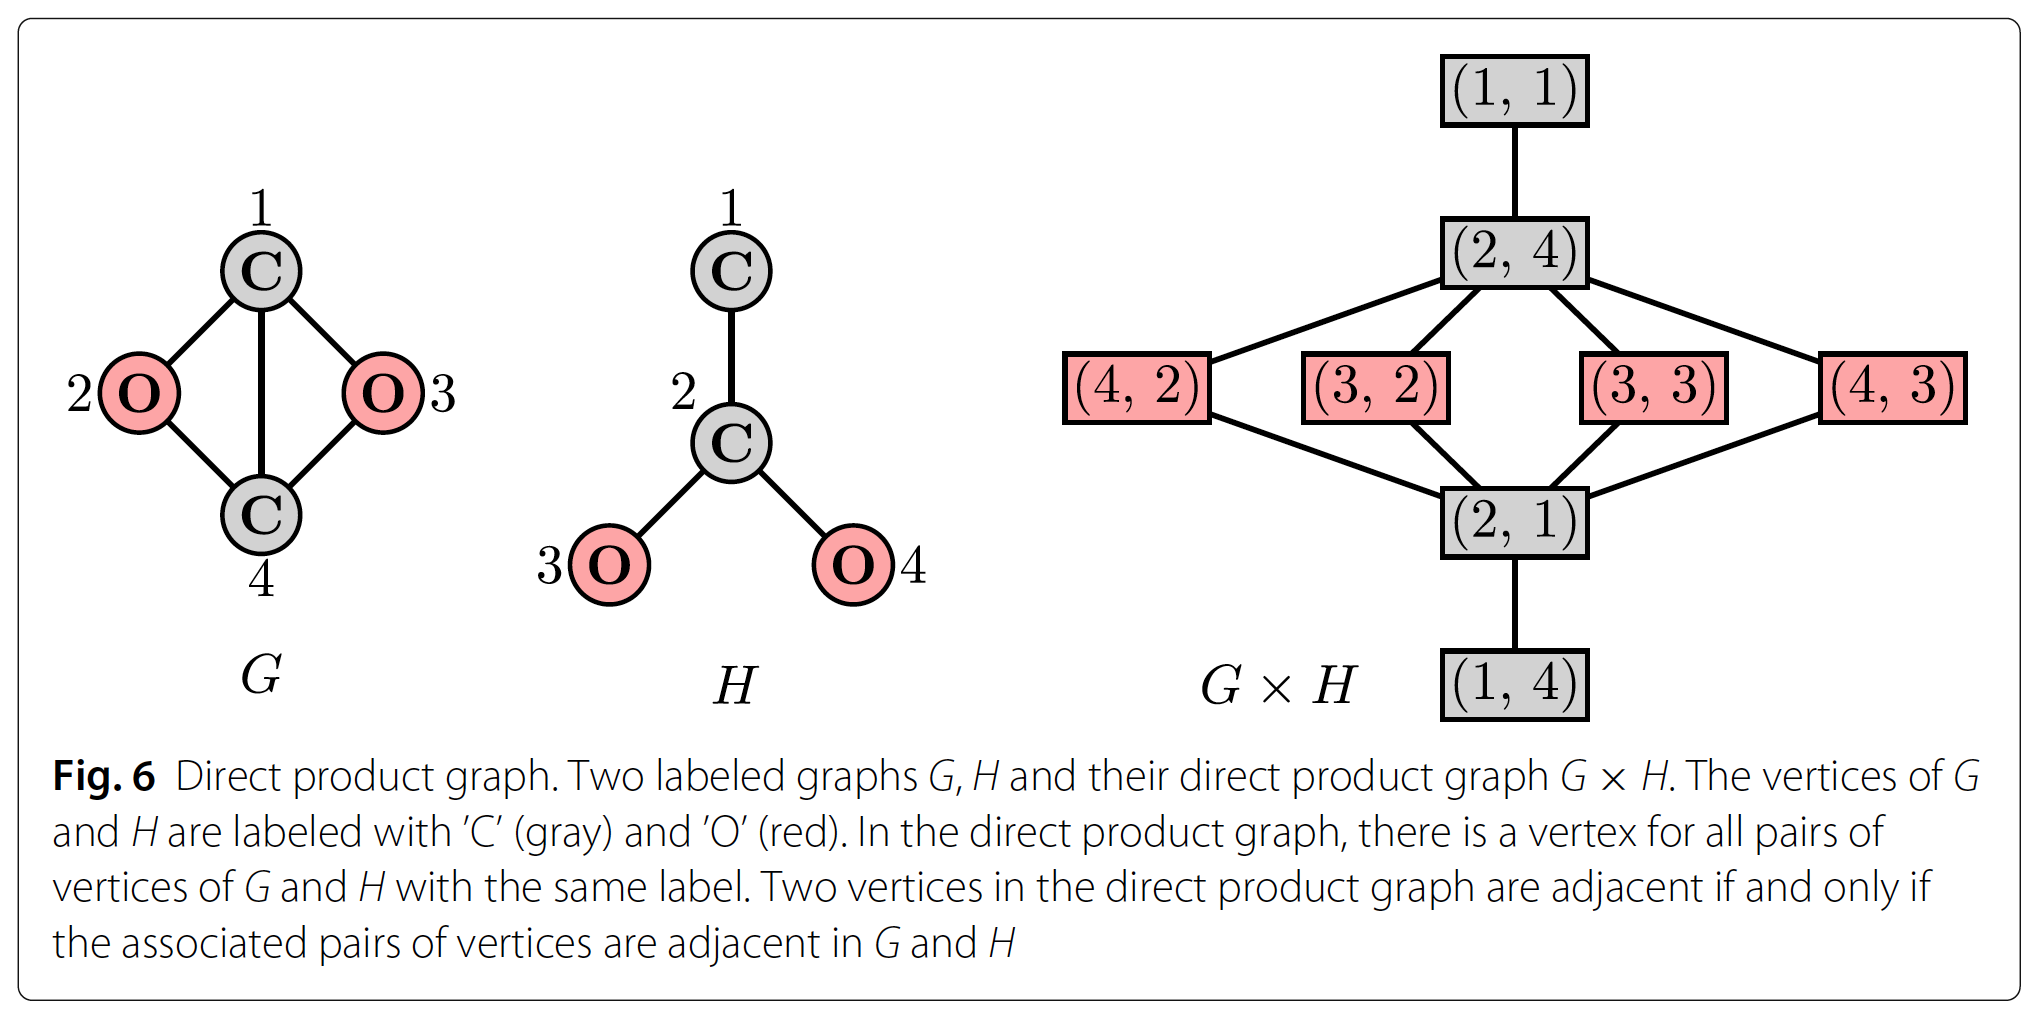
\includegraphics[width=\textwidth]{direct_prod}
	\end{center}
	
\end{frame}
 
\end{document}
